\chapter{Extracción de atributos}
\label{chap:Extraccion de atributos}
\Abstract{En este capítulo se van a desarrollar las herramientas y tecnologías necesarias para la extracción de la altura y posición de cada pieza. De esta forma se dispondrá de toda la información necesaria para que el brazo robótico pueda interactuar con cada pieza.}

El objetivo final de este proyecto es la implantación del sistema de visión artificial en un brazo robótico para que este pueda interactuar con las piezas detectadas. Pero para ello es necesario primero obtener las dimensiones de la pieza, la altura de la pieza, así como la orientación de la misma. En capítulos anteriores se ha visto como obtener la posición de la pieza y sus dimensiones con la ayuda de detectores de objetos. En este capítulo se van a desarrollar las herramientas y tecnologías necesarias para la extracción de la altura y posición de cada pieza. De esta forma se dispondrá de toda la información necesaria para que el brazo robótico pueda interactuar con cada pieza.

\section{Análisis de profundidad}
Como ya se ha mencionado anteriormente, para este proyecto se ha empleado la cámara Intel Realsense D435 \citep{IntelD435}. Esta cámara se caracteriza por contar con múltiples sensores y para este proyecto se va a hacer uso de los sensores RGB y de profundidad. El análisis de la imagen de color ya se ha llevado a cabo en los \autoref{chap:Segmentacion con mascaras de color} y \autoref{chap:Segmentacion con redes neuronales} y en esta sección se va a desarrollar el proceso de análisis de la imagen de profundidad.

El primer paso es la obtención de la imagen de profundidad, este proceso se explica de forma detallada en el \autoref{chap:Comunicacion con la camara}, la imagen devuelta por la cámara tiene una dimensión de 480x480x1 píxeles del tipo entero sin signo de 16 bits. Esto se debe a que el sensor es capaz de medir largas distancias de hasta 10 metros y por ello requiere de 16 bits. Esto para nosotros supone un problema a la hora de representar las imágenes ya que nuestros objetos suelen estar próximos a la cámara y debido a la escala estos son apenas reconocibles al mostrar las imágenes. Es por ello por lo que tras obtener la imagen de profundidad esta se reescala para poder ser mostrada. En el proceso de reescalado se pierde la capacidad de poder detectar objetos de forma precisa a más de un metro, pero por suerte esta situación nunca se da en este proyecto.
	
\begin{figure}[ht]  %Selección de la pieza
  \subfloat{
	\begin{minipage}[c][1\width]{0.49\textwidth}
	   \centering
	   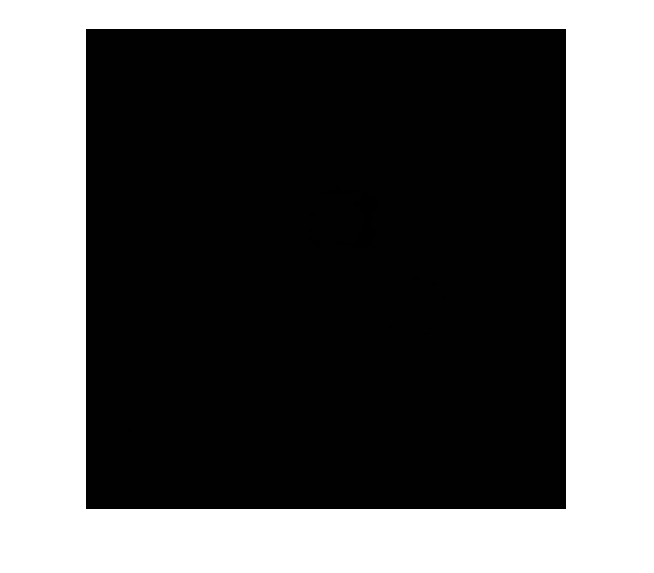
\includegraphics[width=1\textwidth]{Extraccion de atributos/Analisis de profundidad/sin escalado.png}
	\end{minipage}}
  \hfill	
  \subfloat{
	\begin{minipage}[c][1\width]{0.49\textwidth}
	   \centering
	   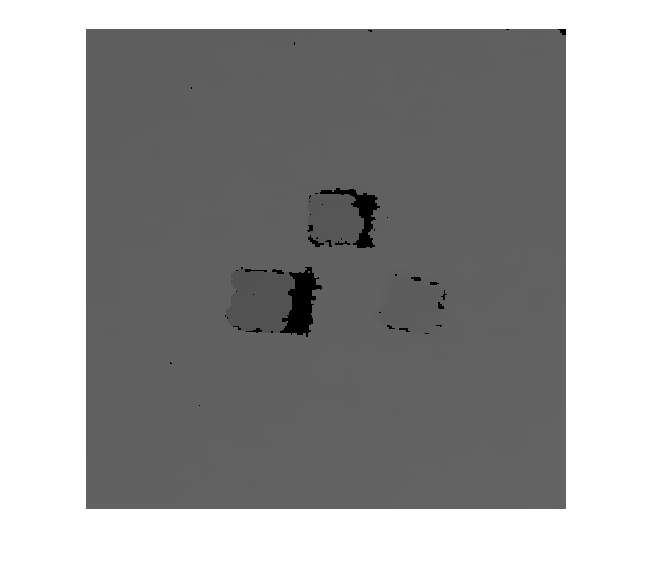
\includegraphics[width=1\textwidth]{Extraccion de atributos/Analisis de profundidad/con escalado.png}
	\end{minipage}}
  \hfill	
\caption{Demostración del escalado de imágenes de profundidad}
\label{fig:Profundidad escaldo}
\vspace{-5pt}
\end{figure}
	
El análisis de profundidad comienza por la calibración de la cámara, para poder trabajar desde diferentes puntos de operación y evitar variaciones en la profundidad por deterioro del \textit{hardware}, es recomendable calibrar la cámara cada vez que se va a usar. El proceso para la calibración es simple y rápida, el objetivo es obtener un mapa de la profundidad del suelo para más adelante poder ser contrastada esta altura con la altura de cada pieza. Para obtener el mapa de profundidad, se divide la imagen de profundidad en 12x12 secciones y se calcula la mediana de profundidad de cada sección. Se ha decidido dividir la zona de trabajo en 12x12 secciones para así reducir la carga del programa y no tener que almacenar en memoria una imagen extra de profundidad. Además, de esta forma se reduce el efecto causado por los reflejos ya que estos se muestran como zonas de profundidad infinita. Se ha decidido emplear la mediana frente a la media debido a su robustez ante valores atípicos. Esto se puede apreciar alrededor de las piezas de LEGO, debido al material y a la orientación de la cara, la cámara no es capaz de detectar correctamente la profundidad y da valores excesivamente grandes o pequeños.
	
Una vez calibrada la cámara, ya se puede empezar a determinar la altura de cada pieza, para ello es necesario haber hallado previamente la posición de todas las piezas. El proceso de obtención de altura es individual e independiente del resto de piezas. El primer paso es obtener la altura media de la pieza recortada y a continuación se contrasta frente al suelo. Teniendo en cuenta el escalado y la altura media de una pieza de LEGO se puede obtener el número de piezas apiladas. A continuación, se muestra un ejemplo en el que se puede observar todo el proceso en la \autoref{fig:Profundidad ejemplo}.

Gracias a la implementación del análisis por secciones, al trabajo con la mediana y al alineamiento de la imagen de profundidad se ha conseguido mitigar notablemente los errores producidos por los reflejos. Esto se debe a que los reflejos distorsionan la imagen de profundidad y hacen que no se pueda obtener la profundidad de las regiones de la imagen afectadas por estos. Al trabajar con secciones la posibilidad de que toda una sección se vea cubierta por un reflejo es baja y por lo tanto es poco probable que no se pueda realizar un análisis de profundidad.

\begin{equation}\label{eq:profundidad}
		altura = (suelo - pieza)* desescalado/20 = (390-330)/20 = 3
\end{equation}

\begin{figure}[ht]
	\centering
	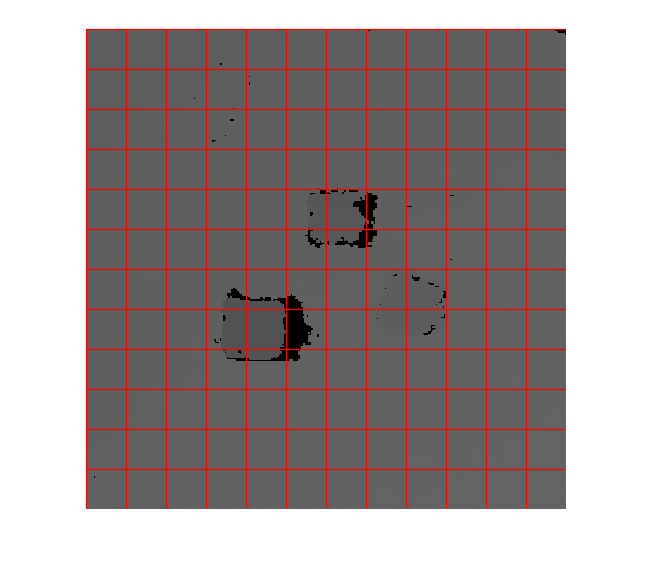
\includegraphics[width=0.7\textwidth]{Extraccion de atributos/Analisis de profundidad/mallado.png}
	\caption{Mallado de imágenes de profundidad para determinación de altura}
	\label{fig:Profundidad mallado}
	\vspace{-5pt}
\end{figure}
	
\begin{figure}[ht]  %Selección de la pieza
  \subfloat{
	\begin{minipage}[c][1\width]{0.49\textwidth}
	   \centering
	   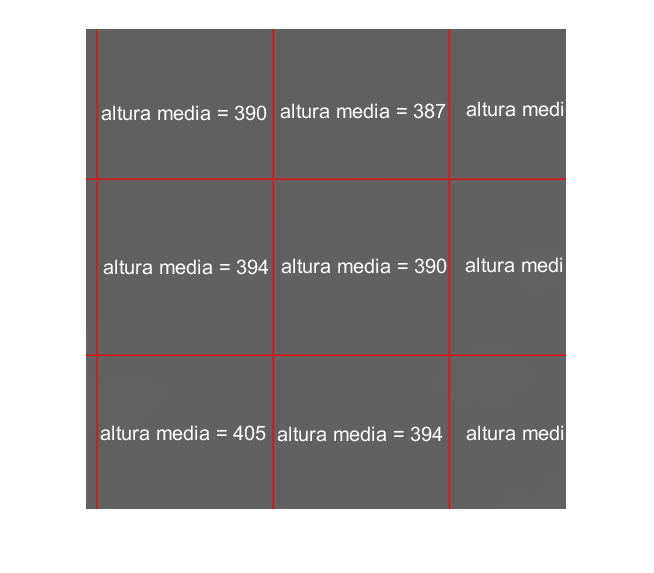
\includegraphics[width=1\textwidth]{Extraccion de atributos/Analisis de profundidad/recorte suelo.png}
	\end{minipage}}
  \hfill	
  \subfloat{
	\begin{minipage}[c][1\width]{0.49\textwidth}
	   \centering
	   \includegraphics[width=1\textwidth]{Extraccion de atributos/Analisis de profundidad/recorte pieza.png}
	\end{minipage}}
  \hfill	
\caption{Demostración del proceso de cálculo de profundidad tras aplicar el desescalado}
\label{fig:Profundidad ejemplo}
\vspace{-5pt}
\end{figure}

\newpage
\section{Análisis de la orientación}
Para poder recoger las piezas con el brazo robótico es necesario saber la orientación de cada pieza. El brazo ha sido programado para orientar su cabezal y pinza de forma que siempre intente coger la pieza de LEGO con un buen agarre pinzando caras planas. El ángulo también nos permite saber si las piezas han sido encajadas en la base del suelo o por el contrario están sueltas. Esta información es vital ya que dependiendo del estado de la pieza, hay diversos métodos por los que el brazo intenta extraer la pieza. Por ello se han desarrollado dos métodos diferentes para la estimación del ángulo.

El primer método a tratar es el método originalmente desarrollado por Ana Berjón Valles \citep{TFGAna} y se basa en la detección de borde y la transformada de Hough. Pero ha sido perfeccionado para mejorar su precisión y evitar situaciones en las que no se pueda detectar ningún borde. El segundo método consiste en el uso de las redes neuronales creadas en el \autoref{chap:Clasificacion con redes neuronales} pero con modificaciones para convertirlas en modelos de regresión basados en redes neuronales.

\subsection{Detección de borde y transformada de Hough}
Tal y como su nombre indica, este método consiste en un análisis empleando la transofrmada de Hough y el algoritmo de paso por cero para la detección de bordes. Los detectores de borde y la transformada de Hough ya han sido ya explicados en la \autoref{subsec:Filtros, detección de borde y detección de formas}. A continuación, se desarrolla el proceso de análisis de una pieza:

\begin{itemize}
\item El primer paso para obtener la orientación de las piezas consiste en aplicar un filtro de color idéntico al visto en \autoref{sec:Filtrado de color} con el fin de obtener una imagen binaria en la que solo se muestren las piezas. Como ya se ha mencionado anteriormente, el filtrado por color presenta grandes problemas de inconsistencia ante cambios de iluminación. Una vez aplicado el filtro se pasa a recortar las piezas y a ser analizas por separado. Este proceso se puede ver en la \autoref{fig:orientación color}.

\item El segundo paso parte de las piezas ya identificadas y separadas. Consiste en aplicar un algoritmo de detección de borde para remarcar solo los bordes exteriores de las piezas. El algoritmo empleado se conoce como paso por cero y se caracteriza porque tal y como su nombre indica, busca los bordes en la imagen que pasen por cero. Es decir, el algoritmo solo resalta las zonas en las que el valor del laplaciano pase por cero ya que son las zonas en las que se producen bordes bruscos. Este proceso se puede ver en la \autoref{fig:orientación bordes}

\item El tercer paso se trata de la transformada de Hough, esta consiste en analizar cada punto de la imagen y hacer pasar por este todos los patrones posibles. Una vez analizados todos los puntos se determinan las relaciones entre estos y se puede extraer información de la forma del objeto.  Este proceso se puede ver en la \autoref{fig:orientacion hough}

\item El cuarto paso trata de analizar la información extraída con la transformada de Hough. En nuestro caso el patrón buscado son rectas, por ello primero se analizará todos los puntos para posteriormente determinar las rectas más importantes y de ellas se extraerá el ángulo. Se puede observar los resultados de este análisis en la \autoref{tab:orientacion hough}
\end{itemize}

Con la ayuda de MATLAB se ha desarrollado un script con el objetivo de comprobar la eficacia de este método. Para ello se han tomado múltiples fotos de piezas de LEGO con una orientación lo más próxima posible a $0^{\circ}$ y se han rotado de forma aleatoria hasta obtener 300 fotos. Con estas fotos se pretende reflejar lo mejor posible la realidad aunque dada las limitaciones físicas y de tiempo las fotos han tenido que ser hechas con un trípode y una cámara réflex. Esto implica que las condiciones no son idénticas a las del laboratorio. Además, la cámara tiene una resolución mucho mayor que la cámara Realsense D435 y esto se refleja en la evaluación. Como el sistema tiene más información los resultados son muy precisos. En la realidad aunque los resultados son buenos, debido a la falta de resolución estos no son tan precisos. Se puede observar en la \autoref{fig:histograma hough} el histograma de las imágenes empleadas para la evaluación.


\begin{itemize}
\item Error medio: Es el error medio cometido al calcular la orientación de todas las piezas. $Error$ $medio = 1.18^{\circ}$
\item Error máximo: Error máximo cometido al analizar las 300 piezas. $Error$ $m \acute{a} ximo = 26^{\circ}$
\item Desviación típica: Representa la dispersión del conjunto de datos. $\sigma = 2.5193^{\circ}$
\item Precisión: Se define como el porcentaje de predicciones cuyo error es inferior a un umbral definido. Se ha decidido que el umbral para determinar el nivel de precisión sea $1^{\circ}$. $Precisi \acute{o} n = 82.67\%$
\item Diagrama de cajas: Permite analizar gráficamente el comportamiento del modelo. Se puede observar el diagrama de cajas en la \autoref{fig:cajas hough} Viendo el primer y tercer cuartil podemos ver que la mayoría de las predicciones tienen un error menor a $1^{\circ}$. También se puede observar la numerosa presencia de valores atípicos. Estos son aquellos cuya desviación sea mayor a 1.5 veces la del recorrido intercuartílico. Se observa hasta un caso con un error de 25 grados.
\end{itemize}

Este método se caracteriza por ser rápido y bastante preciso en la mayoría de las situaciones. Desgraciadamente, no es lo suficientemente constante. Esto se debe al gran número de valores atípicos.

\begin{figure}[ht]  %Primer paso: Filtrado por color para orientación
  \subfloat{
	\begin{minipage}[c][1\width]{0.49\textwidth}
	   \centering
	   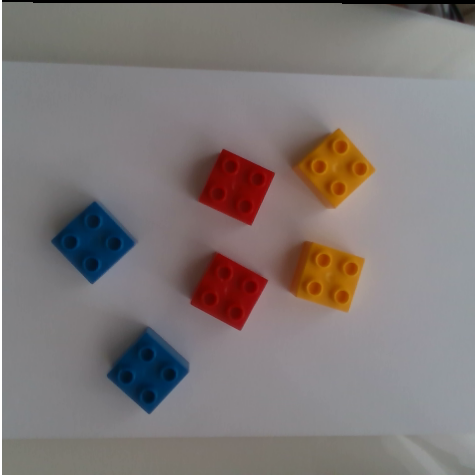
\includegraphics[width=1\textwidth]{Extraccion de atributos/Analisis de orientacion/hough/color.png}
	\end{minipage}}
  \hfill	
  \subfloat{
	\begin{minipage}[c][1\width]{0.49\textwidth}
	   \centering
	   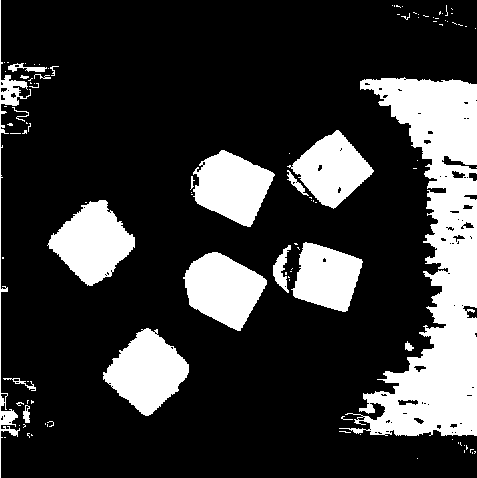
\includegraphics[width=1\textwidth]{Extraccion de atributos/Analisis de orientacion/hough/mascara color.png}
	\end{minipage}}
  \hfill	
\caption[Filtrado por color para el análisis de la orientación]{Primer paso: Filtrado por color para el análisis de la orientación}
\label{fig:orientación color}
\vspace{-5pt}
\end{figure}

\begin{figure}[ht]  %Segundo paso: Selección de la pieza y obtención de bordes
  \subfloat{
	\begin{minipage}[c][1\width]{0.49\textwidth}
	   \centering
	   \includegraphics[width=1\textwidth]{Extraccion de atributos/Analisis de orientacion/hough/recorte pieza.png}
	\end{minipage}}
  \hfill	
  \subfloat{
	\begin{minipage}[c][1\width]{0.49\textwidth}
	   \centering
	   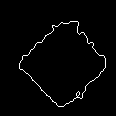
\includegraphics[width=1\textwidth]{Extraccion de atributos/Analisis de orientacion/hough/bordes pieza.png}
	\end{minipage}}
  \hfill	
\caption[Separación y obtención de bordes para el análisis de la orientación]{Segundo paso: Separación y obtención de bordes para el análisis de la orientación}
\label{fig:orientación bordes}
\vspace{-5pt}
\end{figure}

\begin{figure}[ht] % Tercer paso: transformada de Hough
	\centering
	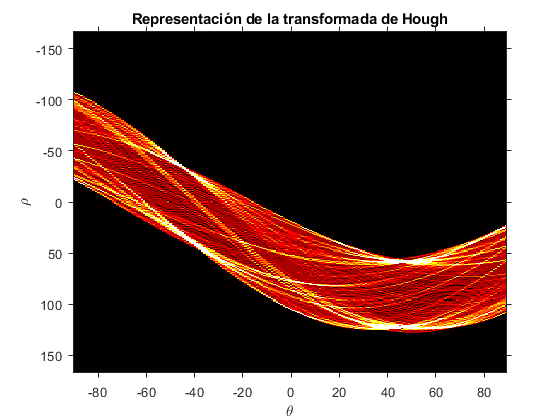
\includegraphics[width=1\textwidth]{Extraccion de atributos/Analisis de orientacion/hough/Hough.png}
	\caption[Análisis de una pieza mediante la transformada de Hough]{Tercer paso: Análisis de una pieza mediante la transformada de Hough}
	\label{fig:orientacion hough}
	\vspace{-5pt}
\end{figure}

\begin{table}[ht] % Cuarto paso: análisis de Hough
  \centering
    \begin{tabular}{|l|l|r|r|}
    \hline
    \multicolumn{1}{|c|}{Punto 1} & \multicolumn{1}{c|}{Punto 2} & \multicolumn{1}{c|}{Theta} & \multicolumn{1}{c|}{Rho}\\
    \hline
    (27,75) & (59,108) & -43   & -31\\
    (49,36) & (62,24) & 45    & 59 \\
    (69,105) & (80,95) & 45    & 122 \\
    (86,88) & (93,82) & 45    & 122 \\
    (101,74) & (106,69) & 45    & 122 \\
    (31,52) & (50,35) & 48    & 58 \\
    (54,31) & (62,24) & 48    & 58 \\
    (41,89) & (51,100) & -46   & -36\\
    \hline
    \end{tabular}%
  \caption[Resultados de la transformada de Hough]{Cuarto paso: Análisis de los resultados de la transformada de Hough y extracción de las rectas más significativas}
  \label{tab:orientacion hough}%
\end{table}%

\begin{figure}[ht] %Histograma de la evaluación
	\centering
	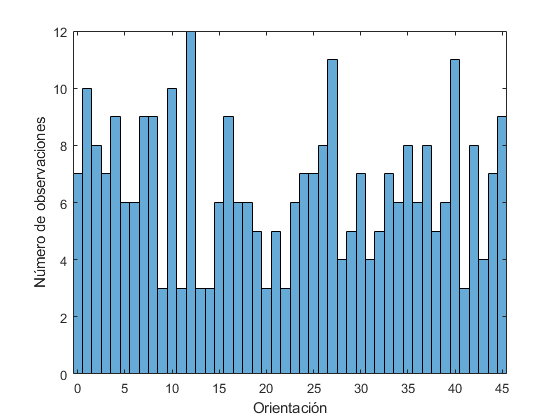
\includegraphics[width=1\textwidth]{Extraccion de atributos/Analisis de orientacion/hough/histograma.png}
	\caption[Histograma de imágenes rotadas empleadas para evaluación]{Histograma de imágenes empleadas para la evaluación del cálculo de la orientación por la transformada de Hough}
	\label{fig:histograma hough}
	\vspace{-5pt}
\end{figure}

\begin{figure}[ht] % Diagrama de cajas
	\centering
	\includegraphics[width=1\textwidth]{Extraccion de atributos/Analisis de orientacion/hough/diagrama de cajas.png}
	\caption[Diagrama de cajas de la orientación por la transformada de Hough]{Diagrama de cajas de la evaluación del cálculo de la orientación por la transformada de Hough}
	\label{fig:cajas hough}
	\vspace{-5pt}
\end{figure}


\clearpage
\subsection{Modelo de regresión con redes neuronales}
Las redes neuronales convolucionales tienen la característica de que pueden ser usadas con múltiples fines. Ya hemos visto en los \autoref{chap:Clasificacion con redes neuronales} y \autoref{chap:Segmentacion con redes neuronales} dos ejemplos de usos para esta tecnología y a continuación, se van a modificar ambos clasificadores ya creados con el objetivo de convertirlos en un modelo de regresión capaz de estimar el ángulo de rotación.

Los modelos de regresión son uno de los primeros usos que se les dio a las redes neuronales y se caracterizan porque la salida no es una clase o la posición de un objeto, en lugar es uno o varios números que representan algún atributo de la imagen. Los modelos de regresión no son exclusivos para el análisis de imágenes, tienen multitud de usos y el uso más común es el análisis estadístico.

\subsubsection*{Preparativos para el entrenamiento y evaluación}
Para el entrenamiento de la red se ha preparado una base de datos con la ayuda de MATLAB. El proceso ha sido la captura de imágenes de alta resolución con piezas de LEGO sin rotación. A continuación, las piezas de LEGO son recortadas de la imagen original y son rotadas múltiples veces. Con esta técnica, se ha conseguido transformar 225 imágenes en un total de 10350 imágenes. Para intentar mostrar todas las posiciones posibles de las piezas de LEGO. Se han tomado fotos en tres escenas diferentes y para cada escena se han tomado 25 fotos para cada pieza de LEGO de color. A continuación, se muestra un montaje con el conjunto de 25 imágenes tomadas para un color en una escena. A todas las imágenes tomadas, se les ha aplicado una rotación para todos los ángulos comprendidos entre $0^{\circ}$ y $45^{\circ}$ y por último se han reescalado al tamaño adecuado para la red. En el caso de LEGONet esta es 227x227 y en el caso de LEGO16 esta es 224x224.

\begin{figure}[ht]
	\centering
	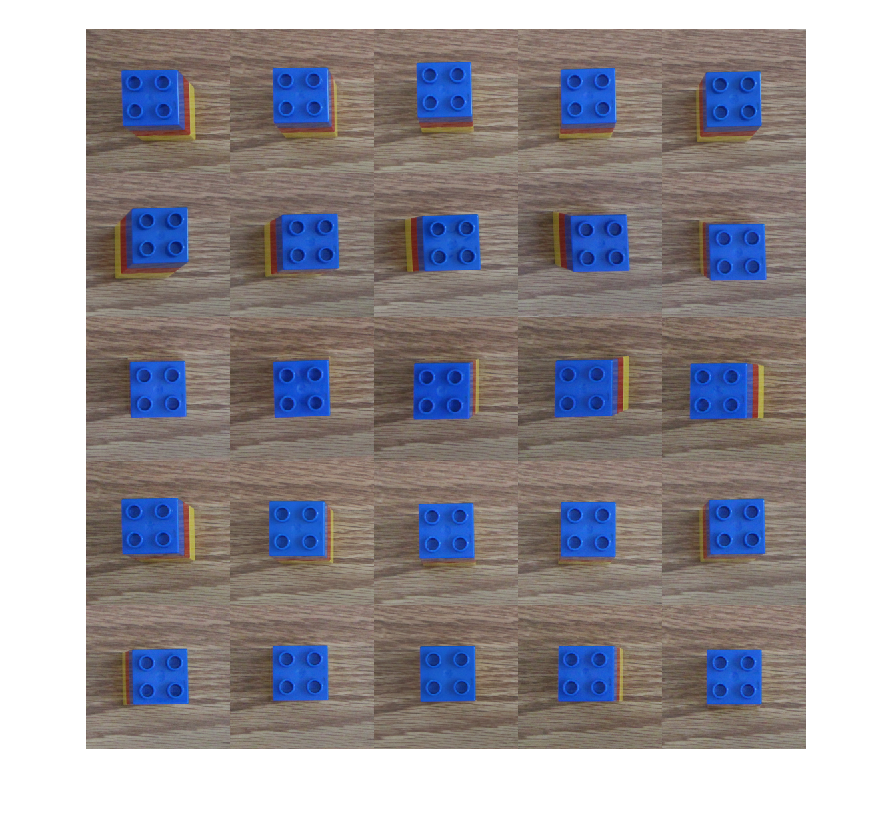
\includegraphics[width=0.5\textwidth]{Extraccion de atributos/Analisis de orientacion/LEGONet/mosaico.png}
	\caption{Imágenes para el entrenamiento de los modelos de regresión}
	\label{fig:regresion LEGONet mosaico}
	\vspace{-5pt}
\end{figure}

\begin{figure}[ht]
	\centering
	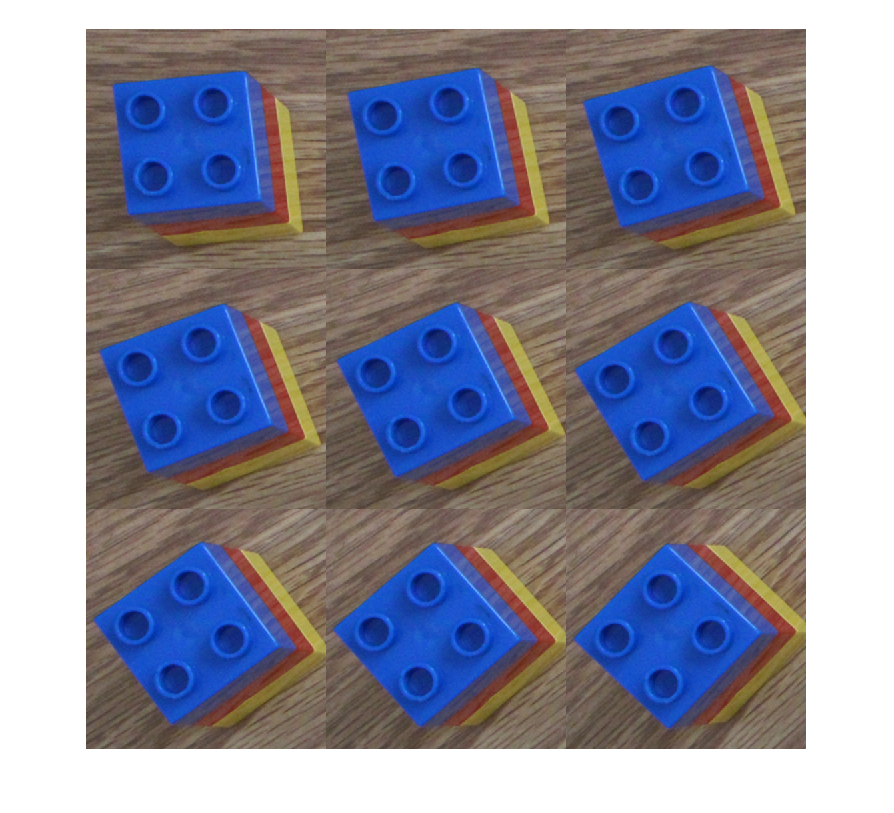
\includegraphics[width=0.5\textwidth]{Extraccion de atributos/Analisis de orientacion/LEGONet/mosaico rotacion.png}
	\caption{Aumento de imágenes para el entrenamiento de los modelos de regresión}
	\label{fig:regresion LEGONet rotacion}
	\vspace{-5pt}
\end{figure}

Con este conjunto de imágenes se ha llevado a cabo el entrenamiento de un modelo de regresión basado en LEGONet y se ha llevado a cabo en un ordenador personal equipado con un i7 4790K, 16GB de memoria RAM y una tarjeta gráfica Nvidia Geforce GTX970 con 4GB de VRAM. Teniendo en cuenta las limitaciones por \textit{hardware} y tiempo, se han realizado múltiples entrenamientos con diferentes opciones de entrenamiento para obtener los mejores resultados. Se ha decidido que el 20\% de las imágenes sean destinadas para validación y el restante para entrenamiento.

Con la ayuda de MATLAB se ha desarrollado un \textit{script} con el objetivo de comprobar la eficacia de este método. Para ello se han tomado 300 fotos de piezas de LEGO con diferentes orientaciones. Con estas fotos se pretende reflejar lo mejor posible la realidad, aunque dada las limitaciones físicas y de tiempo las fotos han tenido que ser hechas con un trípode y una cámara réflex. Esto implica que las condiciones no son idénticas a las del laboratorio. Además, la cámara tiene una resolución mucho mayor que la cámara Realsense D435 y esto se refleja en la evaluación. Como la red tiene más información los resultados son muy precisos. En la realidad, aunque los resultados son muy buenos, debido a la falta de resolución estos no son tan precisos. Se puede observar en la \autoref{fig:histograma redes} el histograma de las imágenes empleadas para la evaluación. En caso de que haya diferencia debido a la diferencia de resolución, esto se puede solventar tomando una foto próxima a la pieza de LEGO.

\begin{figure}[ht] %Histograma de la evaluación
	\centering
	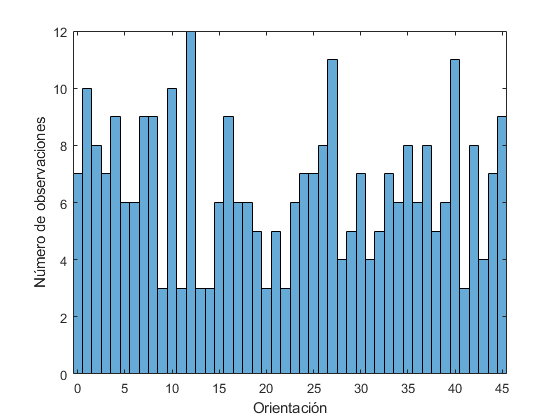
\includegraphics[width=0.7\textwidth]{Extraccion de atributos/Analisis de orientacion/hough/histograma.png}
	\caption[Histograma de imágenes rotadas empleadas para evaluación]{Histograma de imágenes empleadas para la evaluación del cálculo de la orientación}
	\label{fig:histograma redes}
	\vspace{-5pt}
\end{figure}

\subsubsection*{Modelo de regresión basado en LEGONet}
En el \autoref{chap:Clasificacion con redes neuronales} se ha desarrollado un clasificador basado en AlexNet y denominado LEGONet, este al igual que AlexNet cuenta con 13 millones de parámetros y 650.000 neuronas. Para poder reutilizar un clasificador y transformarlo, el primer paso consiste en la eliminación de las tres últimas capas. Es decir, la eliminación de la última capa completamente conectada, la eliminación de la capa \textit{Softmax} y la eliminación de la capa de salida del clasificador. En el caso de LEGONet ha sido necesario eliminar más capas ya que las capas \textit{Dropout} interferían con el entrenamiento. Por ello se ha eliminado todo a partir de la capa relu6 y se ha introducido capas completamente conectadas intercaladas con capas \textit{Batch normalization} y capas \textit{ReLu}. La estructura obtenida se muestra en la \autoref{fig:regresion LEGONet estructura}.

\begin{figure}[ht]
	\centering
	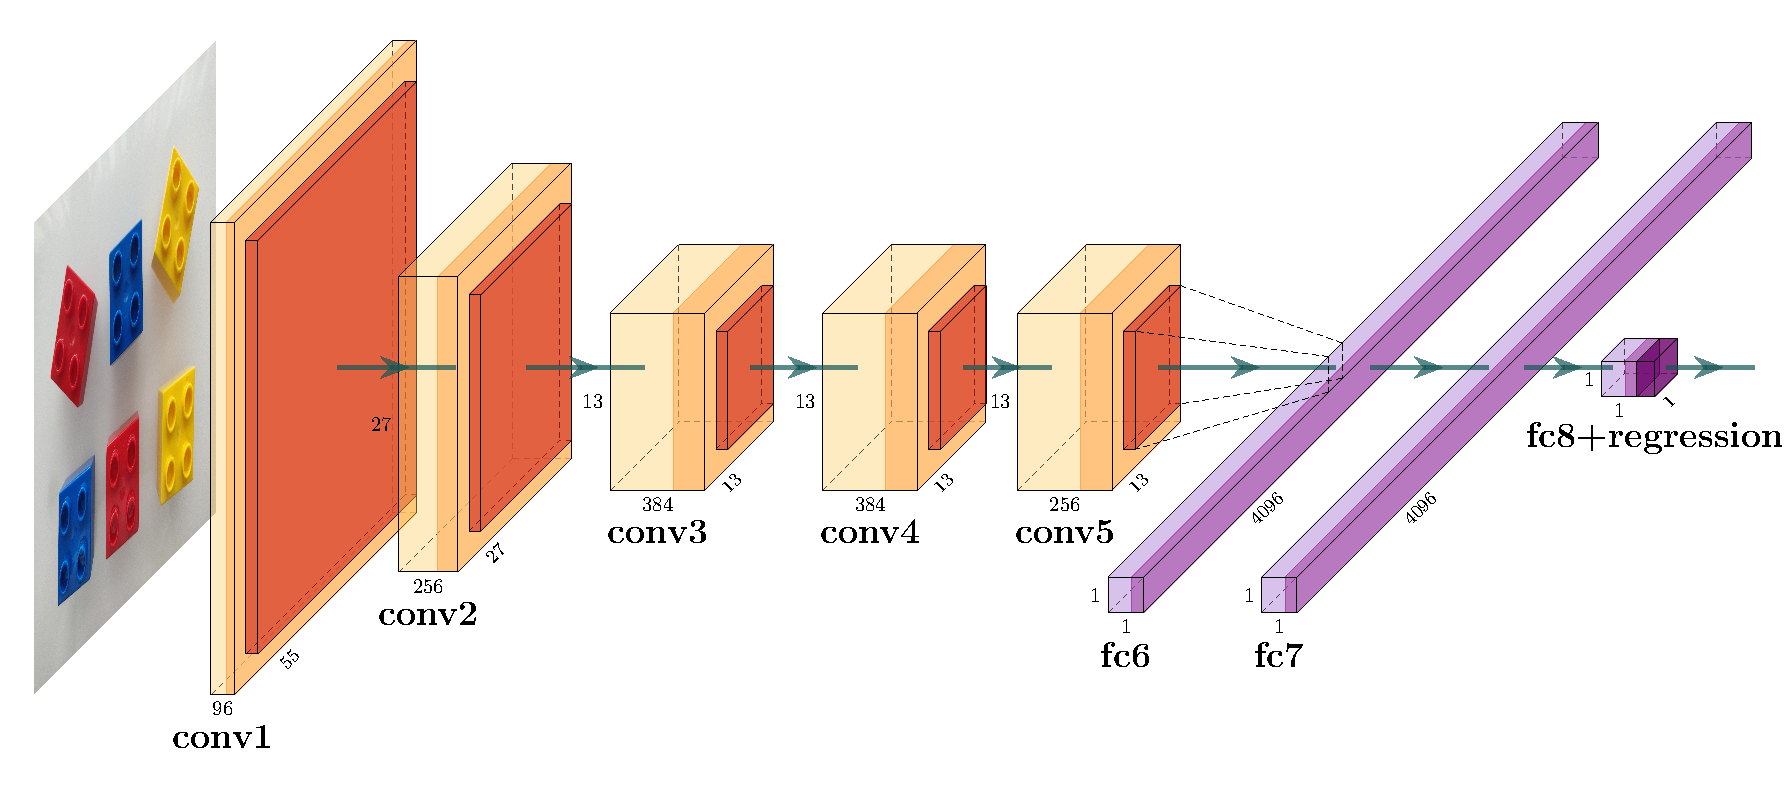
\includegraphics[width=1\textwidth]{Extraccion de atributos/Analisis de orientacion/LEGONet/Regression_LEGONet.pdf}
	\caption{Estructura de un modelo de regresión basado en LEGONet}
	\label{fig:regresion LEGONet estructura}
	\vspace{-5pt}
\end{figure}

Para el entrenamiento de esta red se ha usado la base de datos diseñada en la \autoref{sec:Preparativos para el de entrenamiento detectores}. Esta base de datos consta de un total de 10.350 piezas de LEGO. El 20\% de estas piezas serán empleadas para la validación del entrenamiento. Se han realizado numerosas pruebas de entrenamiento y se ha descubierto que las mejores opciones de entrenamiento son las mostradas en la \autoref{tab:regresion LEGONet options}.

\begin{table}[htbp]
  \centering
    \begin{tabular}{|l|c|}
    \hline
    \multicolumn{2}{|c|}{Opciones de entrenamineto} \\
    \hline
    Solver & \multicolumn{1}{l|}{Stochastic Gradient Descent with Momentum (SGDM)} \\
    \hline
    Momentum & 0.9 \\
    \hline
    Initial Learn Rate & 1.00E-03 \\
    \hline
    Learn Rate Schedule & piecewise \\
    \hline
    Learn Rate Drop Factor & 0.1 \\
    \hline
    Learn Rate Drop Period & 80 \\
    \hline
    L2Regularization & 0.004 \\
    \hline
    Max Epochs & 100 \\
    \hline
    Mini Batch Size & 200 \\
    \hline
    ValidationData & ValidatingData \\
    \hline
    ValidationFrequency & 41 \\
    \hline
    Shuffle data & every epoch \\
    \hline
    \end{tabular}%
  \caption{Opciones de entrenamiento del modelo de regresión basado en LEGONet}
  \label{tab:regresion LEGONet options}%
\end{table}%

Con la ayuda de MATLAB se ha desarrollado un script con el objetivo de comprobar la eficacia de este método. Para ello se van a analizar un total de 300 piezas de LEGO de diferentes colores y con diferentes orientaciones. A continuación, se analizan los resultados obtenidos.

\begin{itemize}
\item Error medio: Es el error medio cometido al calcular la orientación de todas las piezas. $Error$ $medio = 0.3327^{\circ}$
\item Error máximo: Error máximo cometido al analizar las 300 piezas. $Error$ $m \acute{a} ximo = 1.3^{\circ}$
\item Desviación típica: Representa la dispersión del conjunto de datos. $\sigma = 0.4293^{\circ}$
\item Precisión: Se define como el porcentaje de predicciones cuyo error es inferior a un umbral definido. Se ha decidido que el umbral para determinar el nivel de precisión sea $1^{\circ}$. $Precisi \acute{o} n = 97.67\%$
\item Diagrama de cajas: Permite analizar gráficamente el comportamiento del modelo. Se puede observar el diagrama de cajas en la \autoref{fig:cajas LEGONet} Viendo el primer y tercer cuartil podemos ver que la mayoría de las predicciones tienen un error menor a $0.5^{\circ}$. También se puede observar la pequeña presencia de valores atípicos. Estos son aquellos cuya desviación sea mayor a 1.5 veces la del recorrido intercuartílico. Son pocas las situaciones en las que se ha superado un error de $1^{\circ}$ y el mayor error cometido es de $1.3^{\circ}$
\end{itemize}

Este método se caracteriza por ser rápido, aunque depende del número de piezas analizar. Esto se debe a que es necesario correr la red neuronal tantas veces como piezas se hayan detectado. Además de rápido también destaca por ser constante y preciso. De esta forma podemos asegurarnos que el brazo robótico nunca tenga problemas para recolectar las piezas de LEGO.

\begin{figure}[ht] % Diagrama de cajas
	\centering
	\includegraphics[width=1\textwidth]{Extraccion de atributos/Analisis de orientacion/LEGONet/diagrama de cajas.png}
	\caption[Diagrama de cajas de la orientación mediante LEGONet]{Diagrama de cajas de la evaluación del cálculo de la orientación por el modelo de regresión basado en LEGONet}
	\label{fig:cajas LEGONet}
	\vspace{-5pt}
\end{figure}


\subsubsection*{Modelo de regresión basado en LEGO16}
En el \autoref{chap:Clasificacion con redes neuronales} se ha desarrollado un clasificador basado en VGG-16 y denominado LEGO16, este al igual que VGG-16 cuenta con 138 millones de parámetros y 13 millones de neuronas. Para poder reutilizar un clasificador y transformarlo, el primer paso consiste en la eliminación de las tres últimas capas. Es decir, la eliminación de la última capa completamente conectada, la eliminación de la capa \textit{Softmax} y la eliminación de la capa de salida del clasificador. Al igual que con LEGONet, ha sido necesario eliminar más capas ya que las capas \textit{Dropout} impedían el aprendizaje de la red. Por ello se ha eliminado a partir de la capa relu6. Como se ha cortado la red justo después de la primera capa completamente conectada, las primeras capas en añadirse son una capa \textit{Batch normalization} y una capa \textit{ReLu}. A continuación se añaden dos capas completamente conectadas acompañadas también por capas \textit{Batch normalization} y \textit{ReLu}.

En la publicación original de VGG-16 \citep{VGG16} se menciona que descartan el uso de capas \textit{Batch} debido a que en lugar de aportar a la red, entorpecían su entrenamiento. En una primera instancia se intentó hacer lo mismo al crear el modelo de regresión, es decir, no usar capas \textit{Batch}. Desgraciadamente al intentar entrenar estas redes el sistema se negaba a aprender y por ello se optó por la estructura con capas \textit{Batch}.

\begin{figure}[ht]
	\centering
	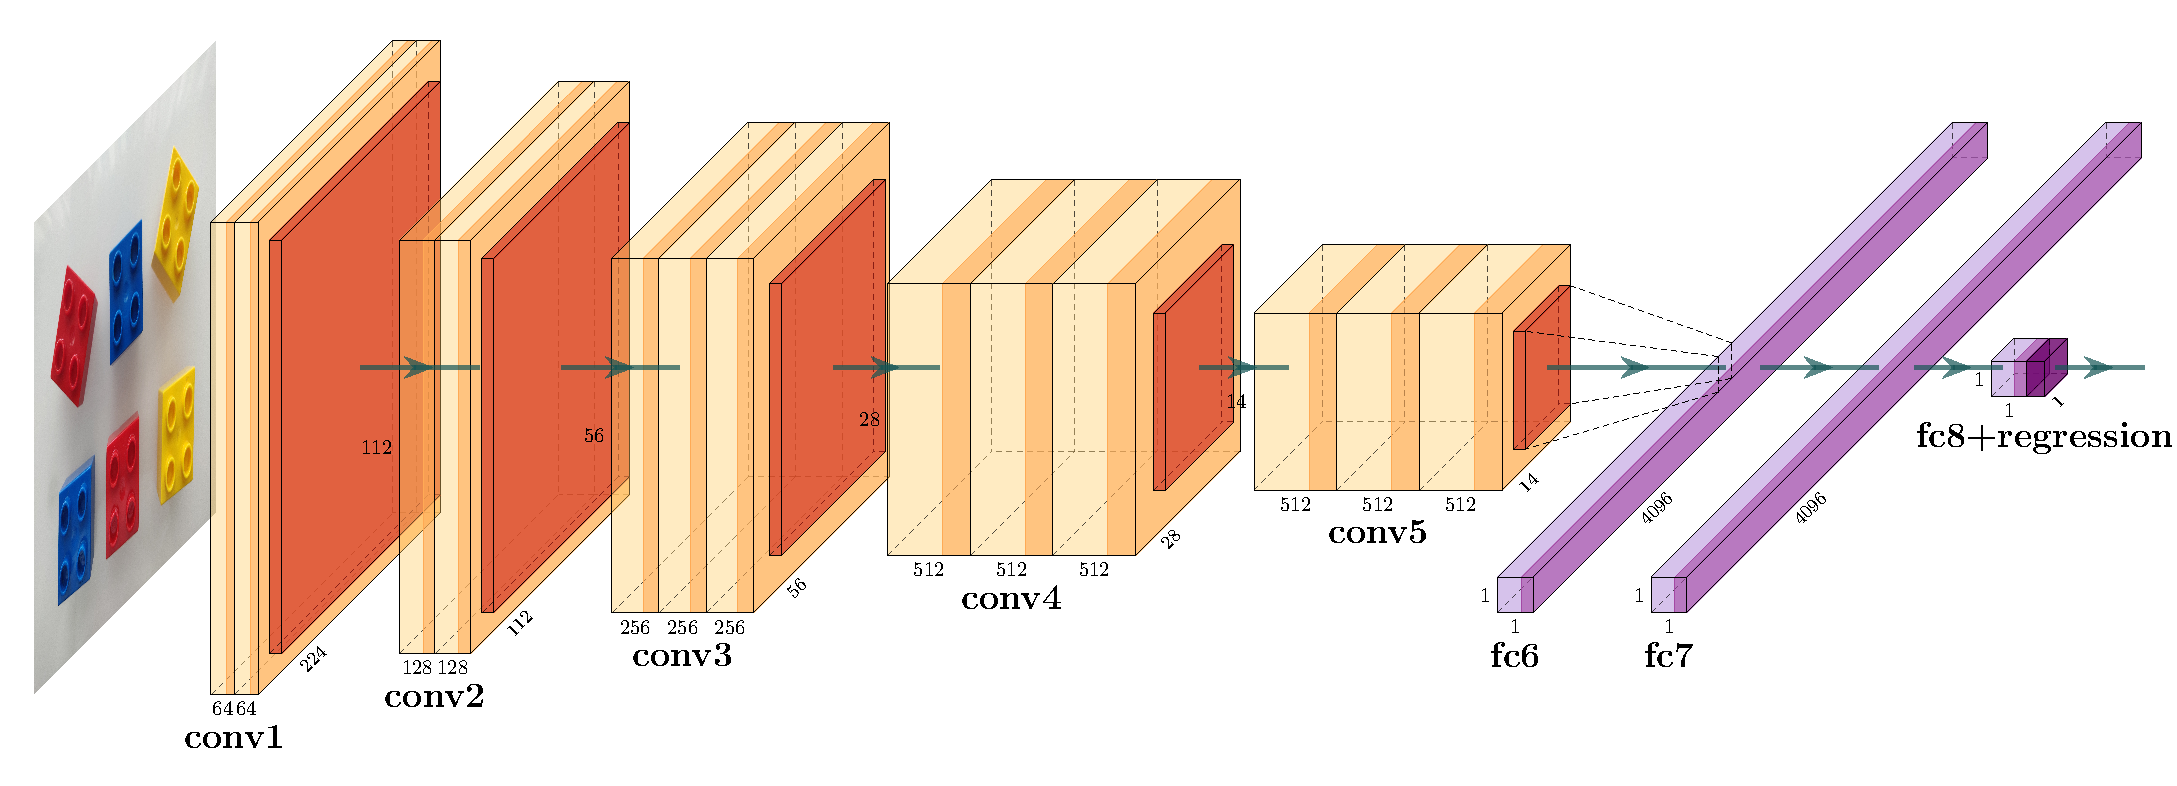
\includegraphics[width=1\textwidth]{Extraccion de atributos/Analisis de orientacion/LEGO16/Regression_LEGO16.pdf}
	\caption{Estructura de un modelo de regresión basado en LEGO16}
	\label{fig:regresion LEGO16 estructura}
	\vspace{-5pt}
\end{figure}

Para el entrenamiento de esta red se ha usado la base de datos diseñada en la \autoref{sec:Preparativos para el de entrenamiento detectores}. Esta base de datos consta de un total de 10.350 piezas de LEGO. El 20\% de estas piezas serán empleadas para la validación del entrenamiento. Se han realizado numerosas pruebas de entrenamiento y se ha descubierto que las mejores opciones de entrenamiento son las mostradas en la \autoref{tab:regresion LEGO16 options}.

\begin{table}[htbp]
  \centering
    \begin{tabular}{|l|c|}
    \hline
    \multicolumn{2}{|c|}{Opciones de entrenamineto} \\
    \hline
    Solver & \multicolumn{1}{l|}{Stochastic Gradient Descent with Momentum (SGDM)} \\
    \hline
    Momentum & 0.9 \\
    \hline
    Initial Learn Rate & 1.00E-03 \\
    \hline
    Learn Rate Schedule & piecewise \\
    \hline
    Learn Rate Drop Factor & 0.1 \\
    \hline
    Learn Rate Drop Period & 7 \\
    \hline
    L2Regularization & 0.004 \\
    \hline
    Max Epochs & 20 \\
    \hline
    Mini Batch Size & 10 \\
    \hline
    ValidationData & ValidatingData \\
    \hline
    ValidationFrequency & 828 \\
    \hline
    Shuffle data & every epoch \\
    \hline
    \end{tabular}%
  \caption{Opciones de entrenamiento del modelo de regresión basado en LEGO16}
  \label{tab:regresion LEGO16 options}%
\end{table}%

Con la ayuda de MATLAB se ha desarrollado un script con el objetivo de comprobar la eficacia de este método. Para ello se van a analizar un total de 300 piezas de LEGO de diferentes colores y con diferentes orientaciones. A continuación, se analizan los resultados obtenidos.

\begin{itemize}
\item Error medio: Es el error medio cometido al calcular la orientación de todas las piezas. $Error$ $medio = 0.7075^{\circ}$
\item Error máximo: Error máximo cometido al analizar las 300 piezas. $Error$ $m \acute{a} ximo = 15^{\circ}$
\item Desviación típica: Representa la dispersión del conjunto de datos. $\sigma = 1.2336^{\circ}$
\item Precisión: Se define como el porcentaje de predicciones cuyo error es inferior a un umbral definido. Se ha decidido que el umbral para determinar el nivel de precisión sea $1^{\circ}$. $Precisi \acute{o} n = 79.33\%$
\item Diagrama de cajas: Permite analizar gráficamente el comportamiento del modelo. Se puede observar el diagrama de cajas en la \autoref{fig:cajas LEGO16} Viendo el primer y tercer cuartil podemos ver que la mayoría de las predicciones tienen un error menor a $1^{\circ}$. También se puede observar que son escasos los casos en los que el error cometido es mayor a $2^{\circ}$. Sin embargo, se ha dado una situación en la que el error es de $16^{\circ}$.
\end{itemize}

Este método se basa en una red neuronal más potente y capaz que LEGONet. Sin embargo, el entrenamiento o la estructura no han sido los adecuados y por ello no llega a superar a LEGONet. Además, al ser una red mayor que LEGONet requiere de más potencia y tiempo de ejecución. Con más tiempo y entrenamiento es posible que se pueda encontrar una red basada en LEGO16 capaz de superar a LEGONet.

\begin{figure}[ht] % Diagrama de cajas
	\centering
	\includegraphics[width=1\textwidth]{Extraccion de atributos/Analisis de orientacion/LEGO16/diagrama de cajas.png}
	\caption[Diagrama de cajas de la orientación mediante LEGO16]{Diagrama de cajas de la evaluación del cálculo de la orientación por el modelo de regresión basado en LEGO16}
	\label{fig:cajas LEGO16}
	\vspace{-5pt}
\end{figure}
